% Document class
\documentclass[10pt, a4paper, twocolumn]{jsarticle}
%
%
% Table of contents fix
\usepackage{atbegshi}
\ifnum 42146=\euc"A4A2
  \AtBeginShipoutFirst{\special{pdf:tounicode EUC-UCS2}}
\else
  \AtBeginShipoutFirst{\special{pdf:tounicode 90ms-RKSJ-UCS2}}
\fi
%
%
% Import packages
\usepackage{amsmath}
\usepackage{amssymb}
\usepackage{bm}
\usepackage{ntheorem}
\usepackage{comment}
\usepackage{ascmac}
\usepackage{float}
\usepackage{subcaption}
\usepackage[dvipdfmx]{hyperref}
\usepackage[dvipdfmx]{graphicx}
\usepackage{enumitem}
\usepackage{multicol}
% \usepackage{fancyhdr}
% \pagestyle{fancy}
% \fancyhf{} % sets both header and footer to nothing
% \renewcommand{\headrulewidth}{0pt}
% \rhead{
%   \begin{tabular}{ll}
%     出願研究科 & 情報科学研究科\\
%     希望研究室 & 情報基盤システム学研究室\\
%     氏   名 & 白石 裕輝\\
%   \end{tabular}
% }
% \cfoot{\thepage}
%
% ----------------------------------------------------------------
% Format
% ----------------------------------------------------------------
% Margin
\usepackage[
  top     = 30truemm,
  bottom  = 20truemm,
  left    = 15truemm,
  right   = 15truemm
]{geometry}
%
\setlength\floatsep{0truemm}						% 図と図の間の余白
\setlength\textfloatsep{-16truemm}				% 本文と図の間の余白
\setlength\intextsep{0truemm}					% 本文中の図の余白
\setlength\abovecaptionskip{0truemm}		% 図とキャプションの間の余白
%
% Caption format (See http://karat5i.blogspot.jp/2014/10/latex.html)
\captionsetup{format=plain, labelformat=simple, labelsep=quad, font=normalsize}
%
% Contents depth
\setcounter{tocdepth}{2}
%
% Page style
% \pagestyle{empty}
%
% Section font
\renewcommand{\headfont}{\bfseries}
%
% Bibliography style
%\bibliographystyle{jplain}
%\bibliographystyle{junsrt}
%
%
% ----------------------------------------------------------------
% Commands
% ----------------------------------------------------------------
% subsubsubsection
  \makeatletter
  \newcommand{\subsubsubsection}{\@startsection{paragraph}{4}{\z@}%
    {1.0\Cvs \@plus.5\Cdp \@minus.2\Cdp}%
    {.1\Cvs \@plus.3\Cdp}%
    {\reset@font\bfseries\normalsize}
  }
  \makeatother
  \setcounter{secnumdepth}{4}
%
% theorem
\newtheorem{Definition}{定義}[section]
\newtheorem{Theorem}{定理}[section]
\newtheorem{Lemma}{補題}[section]
\newtheorem{Proof}{証明}[section]
\newtheorem{Proposition}{命題}[section]
\newtheorem{Axiom}{公理}[section]
\newtheorem{Corollary}{系}[section]
%
% listings
\usepackage{listings, jlisting}
\renewcommand{\lstlistingname}{リスト}
\lstset{
  language=c,
  basicstyle=\ttfamily\scriptsize,
  commentstyle=\textit,
  classoffset=1,
  keywordstyle=\bfseries,
  frame=tRBl,
  framesep=5pt,
  showstringspaces=false,
  numbers=left,
  stepnumber=1,
  numberstyle=\tiny,
  tabsize=2
}
%
% linesparpage
\def\linesparpage#1{\baselineskip=\textheight
  \divide\baselineskip by #1}
%
\makeatletter
  \renewenvironment{thebibliography}[1]{%
    \global\let\presectionname\relax
    \global\let\postsectionname\relax
    \section*{\refname}\@mkboth{\refname}{\refname}%
    \list{\@biblabel{\@arabic\c@enumiv}}%
          {\settowidth\labelwidth{\@biblabel{#1}}%
          \leftmargin\labelwidth
          \advance\leftmargin\labelsep
          % 文字サイズ?
          \setlength\baselineskip{8pt}
          % アイテム間のマージン
          \setlength\itemsep{0.4zh}
          \@openbib@code
          \usecounter{enumiv}%
          \let\p@enumiv\@empty
          \renewcommand\theenumiv{\@arabic\c@enumiv}}%
    \sloppy
    \clubpenalty4000
    \@clubpenalty\clubpenalty
    \widowpenalty4000%
    \sfcode`\.\@m}
    {\def\@noitemerr
      {\@latex@warning{Empty `thebibliography' environment}}%
    \endlist}
\makeatother
%

% argmin, argmax
\newcommand{\argmax}{\mathop{\rm argmax}\limits}
\newcommand{\argmin}{\mathop{\rm argmin}\limits}
%
% ----------------------------------------------------------------
% Title
% ----------------------------------------------------------------
% \title{
%   NAIST において取り組みたい研究
% }
% \author{}
% \date{}
%
%
% ----------------------------------------------------------------
% Document
% ----------------------------------------------------------------
\begin{document}
%
% Make title
\twocolumn[
  \begin{center}
    {\huge NAIST において取り組みたい研究}
    \vspace{4truemm}
  \end{center}
]
%
% Body
\section{はじめに}
\subsection{取り組みたい研究分野}
私は NAIST でオーバレイネットワークに関する研究に取り組みたいと考えている.

\subsection{研究背景}
オーバレイネットワークは IP ネットワークなどのアンダーレイの上位に構築されるアプリケーション層のネットワークである.
オーバレイはアンダーレイにはない機能を持つネットワークを構築することができる.

2000年以降,構造化オーバレイによって実現する分散ハッシュ表 (distributed hash table, DHT) に関する研究が盛んに行われてきた.
DHT とはハッシュ表を複数のノードで分散管理する技術で,ノードの参加や離脱が頻繁に生じるようなネットワーク上でのファイルシステムの構築やメッセージングを可能にする.
大規模な分散システムの耐障害性やスケーラビリティを向上させるために必要不可欠な技術となっている.
特にビッグデータ分析において DHT が果たす役割は非常に大きい.

DHT を実現するアルゴリズムの代表的なものに Chord~\cite{Stoica2001}, Kademlia~\cite{Maymounkov2002} がある.
また,DHT アルゴリズムの根本を見直し,その設計方針を明確にした柔軟な経路表 (flexible routing tables, FRT)~\cite{Nagao2011} という DHT の設計手法がある.
柔軟な経路表によって Chord, Kademlia をそれぞれ再設計した FRT-Chord, FRT-XOR も提案されている.
これらの DHT ではハッシュ関数で決まるノード ID に基づいてトポロジを決定し,ノード数 $N$ に対して $O(\log N)$ の経路長でのルーティングを可能にしている.

構造化オーバレイはアンダーレイのトポロジや通信帯域,ネットワーク近接性などを無視したトラフィックを発生させてしまうという問題点がある.
これに対処するための拡張アルゴリズムも数多く提案されている.

\section{これまでに行った研究}
\subsection{オーバレイに関する研究}
オーバレイではシステムを構成しているノードの通信帯域や処理能力,信頼性などを考慮して適切な役割分担を行うべきである.

私は FRT-Chord に基づき,ネクストホップのノード状態を考慮する構造化オーバレイを提案してきた~\cite{Shiraishi2016}.
これは $O(\log N)$ の経路長とノード状態の考慮を両立するような経路表を構築し,高効率なフォワーディングを可能にするオーバレイである.
実際に,各ノードの最大経路表サイズを考慮する構造化オーバレイを Overlay Weaver~\cite{Shudo2008} 上に実装し,シミュレーション実験を行うことで,フォワーディング効率が向上することを示した.

\subsection{防災情報システムに関する研究}
オーバレイと直接関係はないが,岐阜県情報技術研究所と共同で地理情報システム (geographic information system, GIS) の応用に関する研究も行ってきた~\cite{Shiraishi2014}.
この研究では,GIS への災害情報の登録を効率化するためにスマートフォンの特徴を生かしたアプリを開発した.

従来は県の専門家だけが災害情報の登録を行っていたが,この研究の成果によって登録手順が容易になり,一般の県民も防災リポータとして災害情報を発信できるようになった.
GIS の利用が容易になったことで用途が広がり,県民自らが県民らに情報を発信できる基盤になりつつある.


\section{今後の研究}
\subsection{方針}
構造化オーバレイではアンダーレイのトポロジを考慮し,不要なトラフィックを削減することが望ましい.
そのため,グループ間通信を抑制するアルゴリズムや通信遅延を考慮するアルゴリズムなどが提案されてきたが,複数の状態を同時に考慮するアルゴリズムは提案されていない.

NAIST ではこれまでのオーバレイに関する研究を活かし,ノードの属するグループと通信遅延の両方を同時に考慮する構造化オーバレイの実現を目標に研究を進めようと考えている.

私は経路表構築とルーティングの両者が密接に関係してこそ理想的なオーバレイが実現できると考えている.
そこで,グループ情報を考慮した経路表と通信遅延を考慮した経路表を構築し,これらを用いて適切なルーティングを行うことで複数の状態の考慮を両立しようと考えている.

\begin{figure*}[ht]
  \centering
  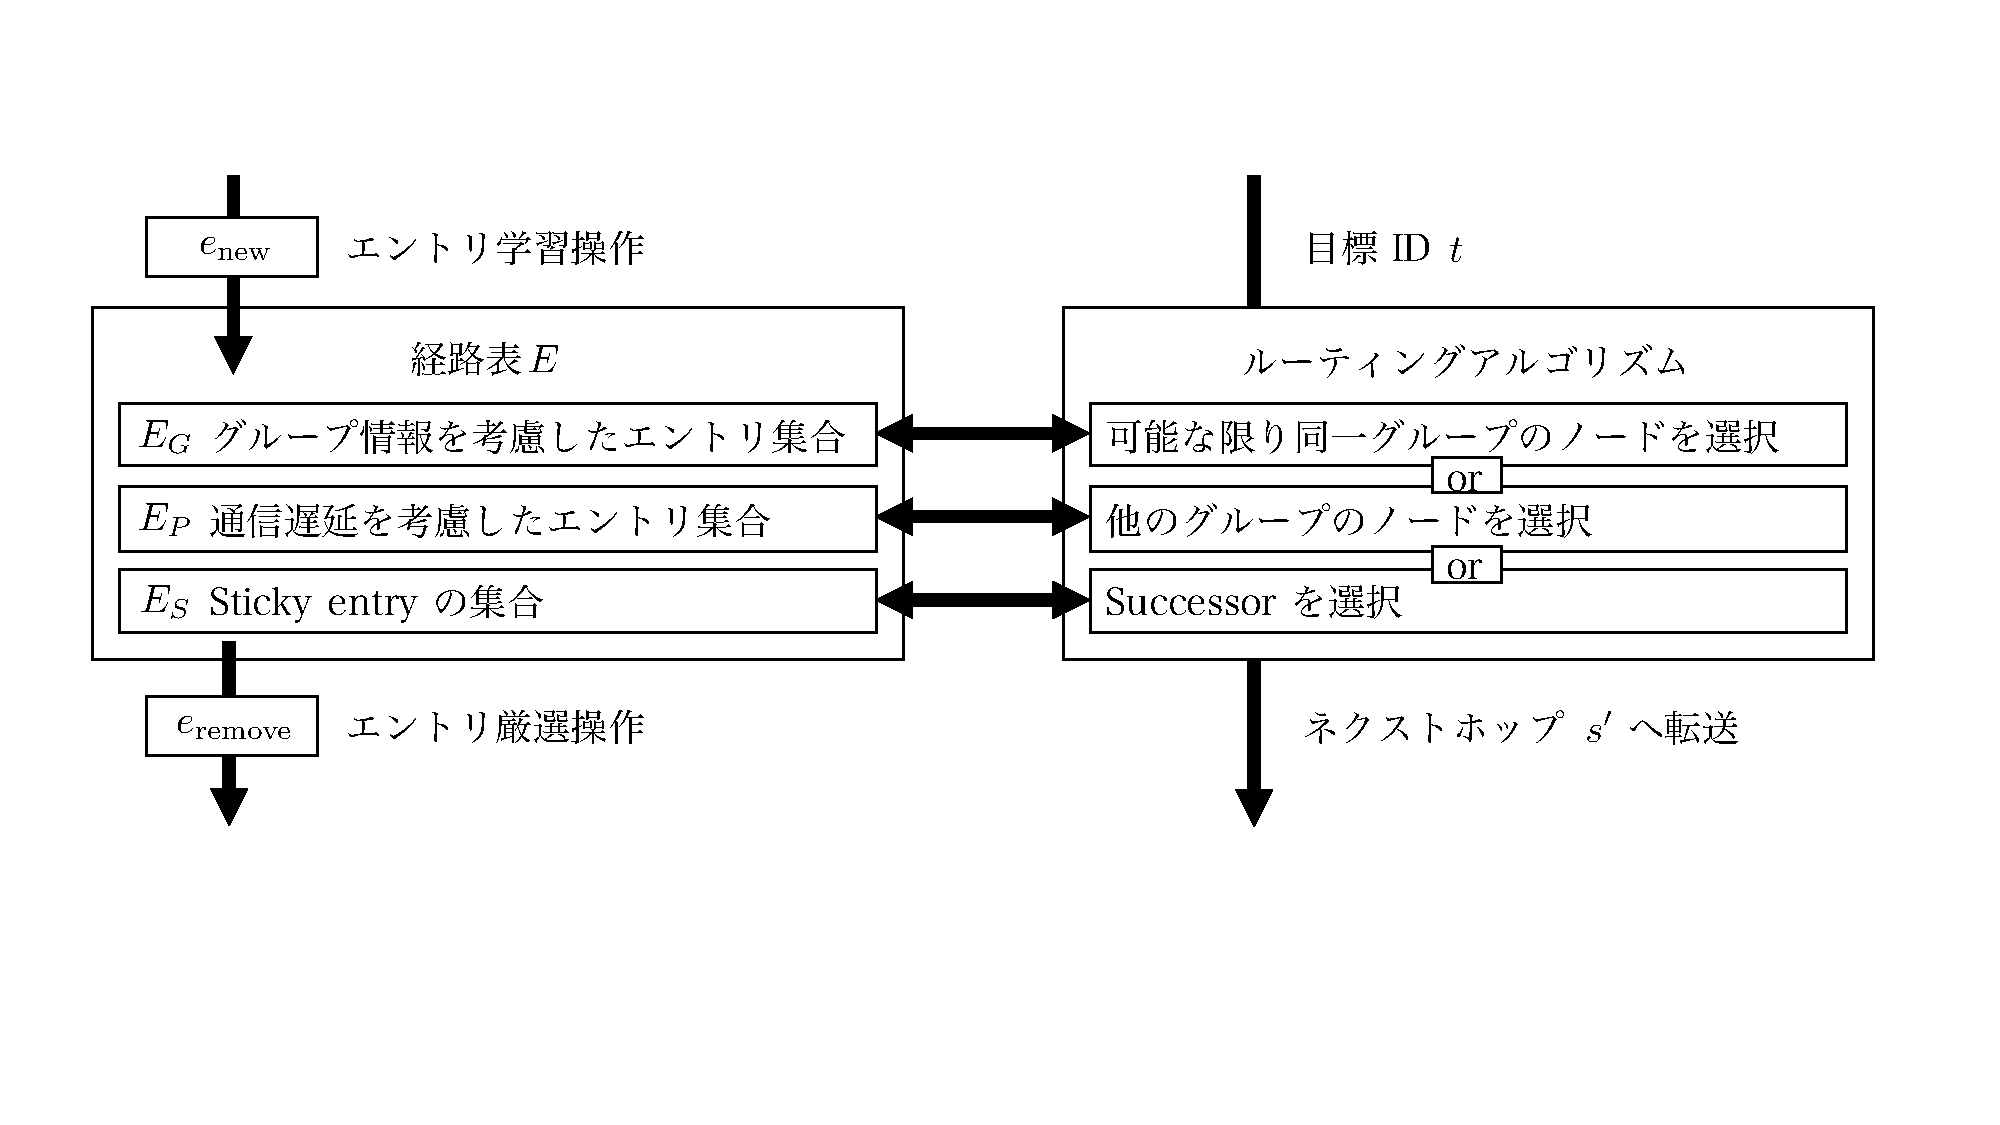
\includegraphics[width=120mm]{fig/str.pdf}
  \caption{提案手法の概要図}
  \label{fig:example}
\end{figure*}

\subsection{提案手法}
FRT-Chord に基づいて DHT を設計する.図\ref{fig:example}に提案手法の概要図を示す.

ノードとオブジェクトにハッシュ関数で決まる ID を与え,consistent hashing に基づいて同一の ID 空間 $P = \{x\ |\ 0 \leq x < 2^m, x \in \mathbb{N}\}$ 上に配置する.ID 間の距離は次のように定義する.
\begin{align}
  \mathrm{d}(x_1, x_2) = x_2 - x_1 \mod 2^m \quad (x_1, x_2 \in P)
\end{align}

各ノードは経路表 $E = E_S \cup E_G \cup E_P = \{e_i\} \ (i = 0, \cdots, |E| - 1)$ を持つ.
経路表のエントリはノード ID と IP アドレスの対で,ネスクトホップの候補である.
$E_S$ は Chord における successor list や predecessor に相当し,到達性を保証する役割を果たす.
$E_G, E_P$ はそれぞれグループ情報を考慮したエントリ集合と通信遅延を考慮したエントリ集合で,構築方法は以降に述べる.

\subsubsection{経路表の構築}
次のエントリ学習操作とエントリ厳選操作を繰り返すことによって,グループ情報を考慮するように $E_G$ を,通信遅延を考慮するように $E_P$ を,そして $O(\log N)$ の経路長を実現するように $E$ を改善する.

\subparagraph{エントリ学習操作}
エントリ学習操作では,ノード $s$ が
\begin{itemize}
  \item 同一のグループに所属する未知のノードと通信したとき新しいエントリ $e_{\mathrm{new}}$ を $E_G$ に,
  \item 同一ではないグループに所属する未知のノードと通信したとき新しいエントリ $e_{\mathrm{new}}$ を $E_P$ に,
\end{itemize}
追加する.
この時,各エントリがノード $s$ からの距離 $\mathrm{d}(s, e_i)$ の昇順に並ぶように追加を行う.

\subparagraph{エントリ厳選操作}
エントリ学習操作で経路表サイズ $|E|$ が最大エントリ数 $L$ を越えようとした時,エントリ厳選操作を行う.

$O(\log N)$ の経路長とグループ情報,通信遅延のすべてを考慮し,$E_G$ もしくは $E_P$ から最も不要なエントリ $e_\mathrm{remove}$ を選択し,削除する.

%ノード $s$ の経路表の各エントリの正規化間隔を次のように定義する.
%
%\begin{align}
%  S^E_i = \log \frac{\mathrm{d}(s, e_{i+1})}{\mathrm{d}(s, e_i)} \quad (0 \leq i < |E| - 1)
%\end{align}
%
%$C = E \setminus E_S$ を考える.$e_{\mathrm{remove}} = \argmin_{e_i \in C} S^{C}_{i-1} + S^{C}_{i}$ を求め,
%
%\begin{itemize}
%  \item $e_\mathrm{remove} \in E_P$ かつ $E_P \setminus \{e_\mathrm{remove}\}$ の平均通信遅延時間が $E_P \setminus \{e_P\ |\ \forall e_P \in E_P\} $ の平均通信遅延時間よりも大きいとき,$e_\mathrm{remove}$ を,
%  \item そうでない場合は
%\end{itemize}


%まず,$E_P$ からエントリ $e_{\mathrm{remove}} = \argmin_{e_i \in E_P} S^{E_P}_{i-1} + S^{E_P}_{i}$ を選び,経路表から削除することで $|E| \leq L$ を保つ.

\subsubsection{ルーティングアルゴリズム}
ノード $s$ から目標 ID $t$ へのメッセージはエントリ (ネクストホップ) $s' = \argmin_{e_i \in E} \mathrm{d}(e_i, t)$ へのフォワーディングを再帰的に繰り返すことで到達する.
このとき,$E_G$ を用いた同一グループ間のフォワーディングで可能な限り目標 ID $t$ への残りの距離を削減し,最終的に $E_P$ や $E_S$ を用いてメッセージを到達させるようにする.

\section{まとめ}
私がこれまでに行ってきた研究と NAIST で取り組みたい研究について述べた.
今後の研究においては,提案手法のエントリ厳選操作とルーティングアルゴリズムの具体的な手順の決定,そしてこれらの評価に取り組んでいきたい.

この研究に取り組むにあたって,NAIST に進学する理由は主に次の2つである.

一つは NAIST の刺激的な環境である.
NAIST は大学院大学であり,「〇〇を研究したい」という明確な目標を持った学生が集まる.
先生方の熱心なご指導を受けながら,周りの活気あふれる学生と切磋琢磨し,充実した研究活動を行うことができると考えている.

もう一つは NAIST の持つ研究設備である.
大規模クラウド実験基盤システムでは,設計したオーバレイを実際に動かし,評価することができる.

私は NAIST の素晴らしい環境の中で,より効率的なオーバレイの実現を目指して研究を行いたいと考えている.


\begin{thebibliography}{9}
    \bibitem{Stoica2001} I. Stoica, R. Morris, et al., ``Chord: A Scalable Peer-to-peer Lookup Service for Internet Applications,'' {\it ACM SIGCOMM '01}, pp. 149--160, 2001.
    \bibitem{Maymounkov2002} P. Maymounkov, D. Mazieres, ``Kademlia: A Peer to Peer Information System Based on the XOR Metric,'' {\it IPTPS '01}, pp. 53--65, 2002.
    \bibitem{Nagao2011} H. Nagao, K. Shudo, ``Flexible Routing Tables: Designing Routing Algorithms for Overlays Based on a Total Order on a Routing Table Set,'' {\it IEEE P2P 2011}, pp. 71--81, 2011.
    \bibitem{Shiraishi2016} 白石 裕輝, 安田 真, ``構造化オーバレイネットワークにおけるノード状態を考慮した経路表構成手法,'' 情報処理学会全国大会論文集, Vol. 78, No. 3, pp. 163-164, 2016.
    \bibitem{Shudo2008} K. Shudo, Y. Tanaka, et al., ``Overlay Weaver: An Overlay Construction Toolkit,'' {\it Comput. Commun.}, Vol. 31, No. 2, pp. 402--412, 2008.
    \bibitem{Shiraishi2014} 白石 裕輝, 西中 智樹他, ``スマートフォン向け岐阜県防災情報システムアプリの開発,'' {\it FIT2014}, Vol. 13, No. 4, pp. 69--74, 2014.
\end{thebibliography}
%
%
\end{document}
